%====================================================================
%Encap�alament
%====================================================================
\documentclass[a4paper,oneside,12pt]{article}
\usepackage[left=2.5cm,right=2cm,top=2cm,bottom=2cm]{geometry}
\usepackage[catalan]{babel}
\usepackage[T1]{fontenc}
\usepackage[latin9]{inputenc}
\usepackage{graphicx} % Required for including pictures
\usepackage{subfigure} % subfiguras
\usepackage{float} % Allows putting an [H] in \begin{figure} to specify the exact location of the figure
\usepackage{wrapfig} % Allows in-line images
\linespread{1.2}
\graphicspath{{Pictures/}}

\usepackage{subscript} %super�ndexs i sub�ndexs
\setcounter{secnumdepth}{5} %Numerar fins a subpar�grafs
\usepackage{pdfpages} %posar arxius pdf (com articles...)

\usepackage{amssymb, amsmath, amsbsy} % librerias ams
\usepackage{stackrel} %Escriure a sobre o sota de qualsevol fletxa
\usepackage{color}
\usepackage{multicol}
\usepackage{array}
\usepackage[full]{textcomp}
\usepackage{multirow}

% Enumeracions
\usepackage[shortlabels]{enumitem}
\usepackage{pstricks}

\usepackage{tikz}
\newcommand*{\itembolasazules}[1]{% bolas 3D 
	\footnotesize\protect\tikz[baseline=-3pt]% 
	\protect\node[scale=.7, circle, shade, ball
	color=blue]{\color{white}\Large\bf#1};}

\newcommand*{\itembolasverdes}[1]{% bolas 3D 
	\footnotesize\protect\tikz[baseline=-3pt]% 
	\protect\node[scale=.7, circle, shade, ball
	color=green]{\color{white}\Large\bf#1};}

\newcommand*{\itembolasrojas}[1]{% bolas 3D 
	\footnotesize\protect\tikz[baseline=-3pt]% 
	\protect\node[scale=.7, circle, shade, ball
	color=red]{\color{white}\Large\bf#1};}

% Lletres gregues
\DeclareRobustCommand{\greektext}{%
  \fontencoding{LGR}\selectfont\def\encodingdefault{LGR}}
\DeclareRobustCommand{\textgreek}[1]{\leavevmode{\greektext #1}}
\DeclareFontEncoding{LGR}{}{}
\DeclareTextSymbol{\~}{LGR}{126}

%Bibliografia
\usepackage[square]{natbib}

% Instruccions especials
\newcommand{\seny}{senyalitzaci�}
\newcommand{\aas}{amino�cids}
\newcommand{\TF}{factor de transcripci�}
\newcommand{\TFs}{factors de transcripci�}
\newcommand{\tgfb}{TGF\textgreek{b}}
\newcommand{\pparg}{PPAR\textgreek{g}}
\newcommand{\betaadren}{\textgreek{b}-adren�rgic}
\newcommand{\Rbeta}{R\textsubscript{\textgreek{b}}}
\newcommand{\iso}{isoproterenol}
\newcommand{\aden}{adenilat ciclasa}
\newcommand{\ca}{Ca\textsuperscript{2+}}
\newcommand{\betacat}{\textgreek{b}-catenina}
\newcommand{\fletsup}{$\uparrow$}
\newcommand{\fletinf}{$\downarrow$}
\newcommand{\gng}{gluconeog�nesi}
\newcommand{\tnfa}{TNF-\textgreek{a}}
\newcommand{\ikb}{I\textgreek{k}B\textgreek{a}}
\newcommand{\nfkb}{NF-\textgreek{k}B}
\newcommand{\pgc}{PGC-1\textgreek{a}}
\newcommand{\na}{Na\textsuperscript{+}}
\newcommand{\pot}{K\textsuperscript{+}}
\newcommand{\ags}{�cids grassos}
\newcommand{\ck}{cicle de Krebs}
\newcommand{\ag}{�cid gras}
\newcommand{\ppara}{PPAR\textgreek{a}}
\newcommand{\ppard}{PPAR\textgreek{d}}
\newcommand{\ifng}{IFN-\textgreek{g}}

% F�rmules qu�miques
\usepackage{chemformula}
%\usepackage[version=4,arrows=pgf]{mhchem}
\usepackage{texshade}
\usepackage{textopo}

%\newcommand{\powd}[1]{$10^{#1}$}
%\newenvironment{?}{?}{?}

\setcounter{tocdepth}{2} % numerar fins subseccions a TOC

% Encap�alament i peu de p�gina
\usepackage{fancyhdr}
\pagestyle{fancy}
%\renewcommand{\sectionmark}[1]{\markright{\textsc{\thesection. #1}}}
\lhead{}
\rhead{}
\lfoot{\sc Malalties gen�tiques}
%\rfoot{\thepage}
\cfoot{}

\fancyfoot[R]{\thepage}

\renewcommand{\headrulewidth}{0.4pt}
\renewcommand{\footrulewidth}{0.4pt}

\raggedbottom
\providecommand{\tabularnewline}{\\}


% Format seccions
%\usepackage{sectsty}
%\sectionfont{\centering\nohang\LARGE\bfseries}
%\partfont{\centering\huge\red}
\usepackage{titlesec}

\titleformat{\section}[block]{\centering}{\bfseries\LARGE\thesection  . }{0em}{\LARGE\bfseries}{}

\titleformat{\subsection}[hang]{\flushleft}{\bfseries\Large\thesubsection }{0.2cm}{\Large\bfseries}

\titleformat{\subsubsection}[hang]{\flushleft}{\bfseries\large\thesubsubsection }{0.2cm}{\large\bfseries}

% Format parts
%\titleformat{\part}[hang]{\centering\vspace{-1.75cm}}{\bfseries\huge\thepart . }{0em}{\huge \bfseries}{}
\newcommand{\titline}{\titlerule[2pt]}
\titleformat{\part}[hang]
  {\vspace{-2cm}\sc\bfseries\huge\red}{\centering\huge\sc\bfseries
  	}
  {0ex}
  {\titline \\
   \vspace{1pt}%
   \centering\huge\sc\bfseries\red\thepart . }
   [%
 \titline]

\usepackage[hyperindex,linktocpage]{hyperref}

% Format �ndex
\usepackage{kpfonts}
\usepackage{titletoc}
\contentsmargin{0cm}
\titlecontents{part}[0pc]
{\addvspace{30pt}%
	\\\color{red}\large\sc\bfseries}%
{}
{}
{\;\titlerule\;\large\bfseries \thecontentspage}%
\titlecontents{section}[2.4pc]
{\addvspace{1pt}}
{\bfseries\contentslabel[\thecontentslabel]{2.4pc}}
{}
{\hfill\small\bfseries\thecontentspage}
[]
\titlecontents*{subsection}[4pc]
{\addvspace{-1pt}\small}
{}
{}
{\ --- \small\thecontentspage}
[ \textbullet\ ][]
%%--


% ====================ENTORNS ====================
\usepackage{tikz,tkz-tab}
\usepackage{tcolorbox, empheq}%

% Entorn per dades
\definecolor{colordadesfons}{RGB}{255,255,255}
\definecolor{colordadesmarc}{RGB}{108, 217, 0}

%\definecolor{colorrecfons}{RGB}{203,216,227}
\definecolor{colorrecfons}{RGB}{255,255,255}
\definecolor{colorrecmarc}{RGB}{128,177,221}

\tcbuselibrary{theorems}
\newtcbtheorem[number within=section]{dades}{An�lisi de dades} {colback=colordadesfons,colframe=colordadesmarc,fonttitle=\bfseries,separator sign={\ $\blacktriangleright$}}{theo}

\newtcbtheorem[number within=section]{rec}{Recordatori} {before=\begin{center},after=\end{center},colback=colorrecfons,colframe=colorrecmarc,fonttitle=\bfseries,separator sign={\ $\blacktriangleright$}}{theo}

\newtcbtheorem[number within=section]{metodes}{M�todes} {colback=red!5!white,colframe=red!75!black,fonttitle=\bfseries,separator sign={\ $\blacktriangleright$}}{theo}

% Equacions
\tcbuselibrary{skins,breakable}
\newcounter{example}
\colorlet{colexam}{red!75!black}

\newtcolorbox[]{myexample}[2][]{%
	empty,title={#1 \thetcbcounter},attach boxed title to top left,
	boxed title style={empty,size=minimal,toprule=2pt,top=4pt,
		overlay={\draw[colexam,line width=2pt]
			([yshift=-1pt]frame.north west)--([yshift=-1pt]frame.north east);}},
	coltitle=colexam,fonttitle=\Large\bfseries,
	before=\par\medskip\noindent,parbox=false,boxsep=0pt,left=0pt,right=3mm,top=4pt,
	breakable,pad at break*=0mm,vfill before first,
	overlay unbroken={\draw[colexam,line width=1pt]
		([yshift=-1pt]title.north east)--([xshift=-0.5pt,yshift=-1pt]title.north-|frame.east)
		--([xshift=-0.5pt]frame.south east)--(frame.south west); },
	overlay first={\draw[colexam,line width=1pt]
		([yshift=-1pt]title.north east)--([xshift=-0.5pt,yshift=-1pt]title.north-|frame.east)
		--([xshift=-0.5pt]frame.south east); },
	overlay middle={\draw[colexam,line width=1pt] ([xshift=-0.5pt]frame.north east)
		--([xshift=-0.5pt]frame.south east); },
	overlay last={\draw[colexam,line width=1pt] ([xshift=-0.5pt]frame.north east)
		--([xshift=-0.5pt]frame.south east)--(frame.south west);},% 
}

\begin{document}

%----------------------------------------------------------
%Portada
%----------------------------------------------------------
\begin{titlepage}

\newcommand{\HRule}{\rule{\linewidth}{0.5mm}} % Defines a new command for the horizontal lines, change thickness here

\center % Center everything on the page
\HRule \\[0.4cm]
{\Huge\bfseries\textsc{Malalties gen�tiques}} \\[0.4cm] % Title of your document
\HRule \\[04cm]
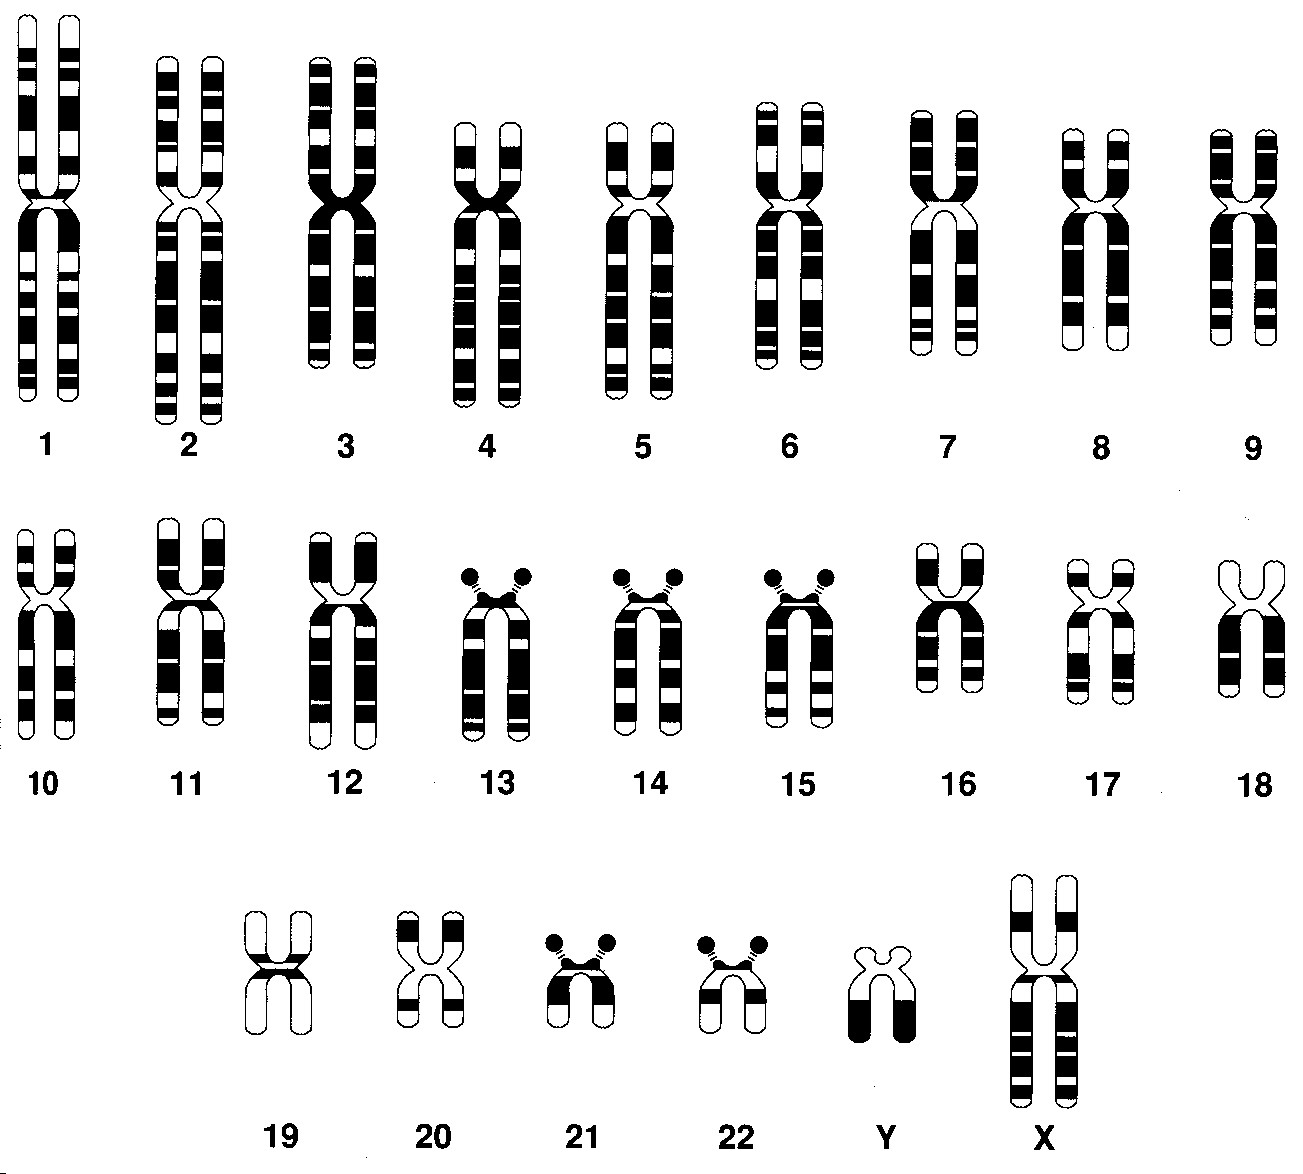
\includegraphics[width=1\textwidth]{Logo} %Include a department/university logo

\vspace{1cm}
\textsc{\Large Ci�ncies Biom�diques UB - Primavera 2017}\\[0.5cm] % Minor heading such as course title
\vspace{0.5cm}
\textsc{\large Albert Torell� P�rez}
\vfill % Fill the rest of the page with whitespace
\end{titlepage}

%===================================
\renewcommand{\figurename}{\textsc{{Figura}}}
\renewcommand{\tablename}{\textsc{{Taula}}}
\renewcommand{\thefootnote}{\alph{footnote}}

%------------------------------------------------------------------------------
%Cos dels apunts 
%------------------------------------------------------------------------------
\pagenumbering{Roman} % para comenzar la numeraci�n de paginas en n�meros romanos

%----------------------------
% Taula de continguts
%----------------------------
\tableofcontents

%--------------------------------------------------------------------------------------------------
%BLOC 1. 
%--------------------------------------------------------------------------------------------------
\newpage
\pagenumbering{arabic}
\part{Introducci�}

%------------------------------------------------------------------------------
% Tema 1. 
%------------------------------------------------------------------------------
%------------------------------------------------------------------------------
% Tema 1. Embrionic Stem Cells
%------------------------------------------------------------------------------
\section{\textit{Embrionic Stem Cells}}
D'una cèl·lula embrionària és interessant obtenir-ne clons. Dels diferents clons que s'obtenen s'ha de comprovar la pluripotencialitat.

Una \textbf{stem cell} és una cèl·lula que presenta 2 propietats (poden ser endògenes o induïdes):
\begin{enumerate}
\item Auto-renovació: es pot dividir de manera que s'obté una cèl·lula idèntica. P.e els fibroblasts presenten aquesta característica. La divisió és simètrica. La capacitat d'auto-renovació depèn de cada clon. El grau d'auto-renovació d'una ESC és dels més alts que es poden aconseguir, en canvi una cèl·lula del mesoderma ja té una capacitat d'auto-renovació més limitada. Una ESC es pot mantenir 1 any \textit{in vitro}. Les cèl·lules mare adultes han perdut la capacitat d'autorenovació.

\item Capacitat de diferenciació: Capacitat de generar una cèl·lula especialitzada per divisió asimètrica (morfologia, patró epigenètic, destí cel·lular). Molts medis de cultiu per cèl·lules mare bloquegen la capacitat de diferenciació.
\end{enumerate}

\subsection{Blastocist pre-implantacional}
Aquest blastocist no està adherit a l'úter, ja que quan s'adhereix a l'úter pateix canvis de morfologia, llinatges, importants. És aproximadament als 5 dies de gestació. S'obtenen cèl·lules de l'estadu entre massa interna i la generació dels 3 fulls embrionaris. Si la massa interna es deixa desenvolupar, es comença a diferenciar. Es força a que la massa interna sigui una \textit{stem cell}.

No totes les ESC són capaces de generar cèl·lules de línia germinal.

Hi ha diferents graus de potència:
\begin{description}
\item[Totipotents] Són els zigots. Poden donar lloc a un organisme sencer ben format. Té una capacitat proliferativa il·limitada i pot desenvolupar tots els teixits i òrgans post-embrionaris

\item[Pluripotents] Són les ESC, del blastocist... Tenen la capacitat d'originar varietats de tipus cel·lulars i teixits.

\item[Multipotents] P.e les cèl·lules mesenquimals. Especialitzades en originar únicament determinats tipus cel·lulars de determinats teixits.
\end{description}

Les \textit{germinal stem cells} també tenen potència. Les iPSC són cèl·lules adultes que s'han desdiferenciat artificialment amb un alt grau de potència.

Les cèl·lules de la medul·la òssia són cèl·lules mesenquimals i hematopoiètiques.

Temple, Nature Reviews Neuroscience, 2005

\subsubsection{Experiments quimera}
Tenen per objectiu demostrar si les cèl·lules són pluripotents o no.

S'obtenen 2 tipus cel·lulars d'un animal que expressa constitutivament la fosfatasa alcalina. Després s'injecten en un blastocist pre-implantacional i es col·loquen en una mare receptora (el grau d'implantació és molt petit). Es recullen els embrions a E11 i es revela l'activitat fosfatasa alcalina.

Si tots els teixits presenten coloració, estem parlant que les cèl·lules injectades són embrionàries.
Si no tots els teixits presenten coloració, vol dir que la potència d'aquestes cèl·lules és més limitada.

En ESC, el control de la divisió cel·lular és molt complicat.

\subsection{Obtenció de cèl·lules mare}
Es poden obtenir per 3 procediments:
\begin{enumerate}
\item Aïllament de la massa cel·lular interna
\item Aïllament de cèl·lules primmordials de l'embrió
\item Transferència nuclear a partir de cèl·lules somàtiques adultes
\end{enumerate}

Aquestes tècniques han evolucionat en paral·lel a FIV.

Un teratoma és un tumor sòlid que conté cèl·lules proliferatives de les 3 capes embrionaries. Per generar els teratomes, s'injectaven les cèl·lules a escrot de ratolí o subdèrmic. Les iPSC tenen la capacitat de produir teratomes.

Quan s'aïlla la massa interna, no s'obté de manera pura. El cultiu pretén recrear les condicions del blastocist. Si són humanes, es plaquegen sobre una capa de fibroblasts irradiats que donen suport físic i biològic (factors de creixement, citocines). El fibroblasts són de prepuci de ratolí, són línies establertes que aguanten molt bé la irradiació. Passats uns dies, es forma un cos embrioide. S'agafen cèl·lules de la perifèria, les cèl·lules del centre estan en hipòxia i les cèl·lules del voltant es diferencien per l'acció del ROS. Aquestes cèl·lules de la perifèria es passen a una altra placa i així successivament fins que s'obtenen clons de ESC.

En el ratolí, hi ha un punt que no es requereix la capa de fibroblasts.



%=================================================================
%=================================================================
\newpage
\phantomsection
\addcontentsline{toc}{part}{Refer�ncies}
\begin{multicols}{2}
\bibliography{bibmalalties} 
\bibliographystyle{authordate3}
\end{multicols}

\end{document}
Avaluaci� continuada: Test de seguiment de la part del Francesc. Tamb�
hi ha un seminari + test (persona externa). Treball online per obtenir
informaci� sobre malalties gen�tiques (OMIM). Cada activitat val un
5\% i l'examen val 35\%.

Part Daniel Grinberg: 15\% de seminaris i 35 d'examen. Els seminaris
consisteixen en la presentaci� i discussi� de papers. Grups de 2/ 2
grups per dia.
